\chapter{Introduction}

The existence of additional $U(1)$ gauge symmetries of nature are common in
several Beyond the Standard Model (BSM) theories \cite{goodsell2010, 
candelas1985, andreas2013, jaeckel2010}. Such theories envision the associated
gauge boson ($A'$, ``dark'', ``hidden'', ``heavy'' photon) inhabiting a hidden sector
consisting of a complex of particles and gauge bosons.  Probing the 
structure of such a hidden sector may be possible through several different portals
including ``kinetic mixing''.  In fact, it is natural for the $A'$ to 
kinematically mix with the Standard Model (SM) photon through the interaction
of massive fields carrying both SM hypercharge and dark charge \cite{holdom1986}.
The mixing of the photon with the $A'$ would not only allow searching for
new hidden sector particles, but also dark matter which some theoretical models
have envisioned as inhabiting the hidden sector, with it's interactions mediated
via an $A'$ \cite{arkani-hamed2009, pospelov2009, cheung2009, arkani-hamed2008}.

The chapter that follows will motivate the need to search for an $A'$, and it's
connection to dark matter.  Furthermore, an overview of current experimental 
searches for an $A'$ will be given.

\section{Physics Motivation}

As Holdom \cite{holdom1986} realized in the mid eighties, in a theory with 
$U(1)_Y \times U(1)'$, there is a term in the gauge part of the Lagrangian 
that allows $U(1)_Y$ and $U(1)'$ to mix.  The gauge part of such a theory can
be written as
\begin{equation}
    \mathcal{L}_{\text{gauge}} = - \frac{1}{4} F_Y^{\mu \nu}F_{Y, \mu \nu}
                          - \frac{1}{4} F'^{\mu \nu}F'_{\mu \nu}
                          + \frac{1}{2} \epsilon F'^{\mu \nu} F_{Y, \mu \nu}
    \label{eqn:l_gauge}
\end{equation}
%the associated gauge boson (heavy photon,
%dark photon or $A'$) can couple to the SM photon through the ``kinetic mixing''
%interaction
where $F'_{\mu \nu} = \partial_{\mu}A'_{\nu} - \partial_{\nu}A'_{\mu}$ 
($F^{\mu \nu}_{Y} = \partial^{\mu}A^{\nu} - \partial^{\nu}A^{\mu}$) is the
field strength tensor of the heavy photon (SM hypercharge) and $\epsilon$ is a
dimensionless coupling constant.  Decoupling of the fields can be achieved by 
shifting the SM hypercharge gauge field as 
\begin{equation}
    A_{\mu} \rightarrow A_{\mu} - \epsilon A'_{\mu}.
\end{equation}
Dropping all $\epsilon^2$ terms, this results in the diagnolization of \ref{eqn:l_gauge} as
\begin{equation}
    \mathcal{L}_{\text{gauge}} = - \frac{1}{4} F_Y^{\mu \nu}F_{Y, \mu \nu}
                          - \frac{1}{4} F'^{\mu \nu}F'_{\mu \nu}.
\end{equation}
However, the redefinition of the field also affects the interaction term of 
the Lagrangian, $\mathcal{L}_{int} = A^{mu}J_{\mu}^{EM}$, which, in turn, induces
an effective coupling between the electromagnetic current and the heavy photon
field that is suppressed by a factor of $\epsilon$
\begin{equation}
    A^{\mu}J_{\mu}^{EM} \rightarrow (A^{\mu} - \epsilon A'^{\mu})J_{\mu}^{EM}
\end{equation}
As explained in chapter 2, this interaction can be exploited to search for heavy 
photons.

An interaction between between the SM photon and the heavy photon can be 
generated at multiple loops assuming there exist a particle, $\Phi$, that is charged
under both the SM hypercharge and dark charge (see Fig. \ref{fig:ap_loop}).
\begin{figure}
    \centering
    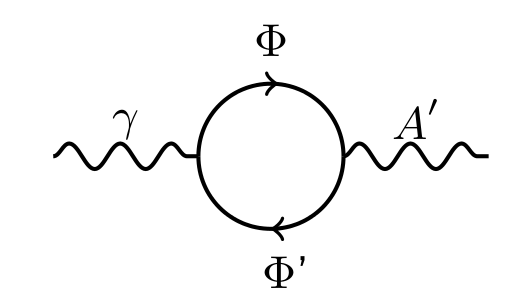
\includegraphics[width=0.5\textwidth]{images/aprime_loop.png}
    \label{fig:ap_loop}
\end{figure}
This generates values of $\epsilon \sim 10^{-8} - 10^{-2}$ 
\cite{arkani-hamed2008, bjorken2009}.  In some string theory constructions, 
values of epsilon as small as $\epsilon \sim 10^{-12}$ are expected \cite{}.

%
% If I have time, I need to add a paragraph explaining how an A' would acquire
% mass.
%

\section{Motivations for a Heavy Photon from Dark Matter}

Although the existence of dark matter (DM) has been firmly established through its
gravitational interaction \cite{popolo2014}, its exact nature continues to elude
us. An appealing
possibility is that DM inhabits a ``hidden sector'' with it's interactions 
mediated by an $A'$.  In turn, the kinetic mixing of the $A'$ with the SM 
photon may provide a portal that would allow the exploration of not only the 
properties of DM but the hidden sector itself.  Furthermore, several recently
observed astrophysical anomalies \cite{pamela2008, ackermann2012, aguilar2013}
may have a dark matter interpretation if it's
charge under an $A'$.  A summary of those anomalies along with their dark matter
interpretation will be presented here.

\subsection{Cosmic Rays}

Interest in hidden sector models surged in 2008 with the announcement by 
The Payload for Antimatter Matter Exploration and Light-nuclei Astrophysics \\ 
(PAMELA) of an unforeseen rise in the ratio of the cosmic ray (CR) positron flux
to CR electron flux, $e^{+}/(e^{+} + e^{-})$, above 10 GeV \cite{pamela2008}.
The rise was later confirmed by both the 
Fermi Gamma-Ray Space Telescope \cite{ackermann2012} and Alpha Magnetic 
Spectrometer-02 \cite{aguilar2013} experiments and observed to continue
up to 200 GeV. 

The main source of CR positrons 
was expected to come from the interaction of CR nuclei with the interstellar 
medium (secondary production).  If such a production mechanism was dominant, 
cosmic ray propagation models predicted the fraction would fall with increasing
energy.  The observed rise lead to the speculation of additional sources of 
positrons including pulsars\cite{} and supernovas\cite{}.

One attractive scenario that could account for the rise was the annihilation of
DM.  Specifically, models where DM annihilates to leptons ($e^+e^-, \mu^+\mu^-$)
where found to fit the data fairly well, although, they
require very large annihilation rates \cite{cholis2009}. Alternatively, a 
more attractive model envisioned DM annihilating to a heavy photon which 
subsequently decays to 
$e^+e^-$ naturally leads to an enhancement in the annihilation cross-section
\cite{arkani-hamed2009}.  This model became less favorable as higher
precision measurements of the positron flux became available.  In fact, 
recent measurements of the cosmic microwave background (CMB) have put very 
tight constraints on such a scenario.

\subsection{Light Dark Matter}

Recently, an analysis of three years of data collected by the Fermi Large Area
Telescope observed an extended emission in the spectrum of gamma-rays 
originating from the Galactic Center \cite{}.  Several models have been 
devised to try to explain the emission including the collision of energetic 
protons accelerated by a super-massive black hole \cite{}, pulsars \cite{} and
dark matter annihilation to leptons or hadron \cite{}.  The emission can also
be explained in the context of dark matter annihilation to an $A'$ which 
subsequently decays to SM particles.  Such a model requires a dark matter 
candidate of mass $\sim$ 10 GeV and heavy photons with a mass in the range 
of $\sim$ 100 MeV. 

Another anomalies that can be explained in the context of a light dark matter
candidate whose interactions are mediated by a heavy photon is the observance
of a 3.5 keV emission line from a cluster of galaxies \cite{}.  In this case, 
dark matter is assumed to self-interact producing an excited state.  The excited
state then decays to it's unexcited state a photon with an energy equal to 3.5 keV.
Again, this requires a $\sim$ GeV dark matter and a $\sim$ GeV mediator.

\section{Current Limits on Heavy Photons}

\subsection{Electron Beam Dump Experiments}

Electron beam dump experiments make use of a high intensity beam ``dumped'' onto
a thick ($\sim$ cm) target to produce highly boosted neutral particles through a 
process analogous to photon bremsstrahlung.  In order to suppress the large
SM backgrounds produced at the target, a shield of thickness ($\sim$ cm - m)
is usually placed immediately downstream and in front of the detector.
% What backgrounds are these experiments concerned with?
% What is the shield made of?
The thickness of the target and shield in combination with the high luminosities
resulting from the intense beams allow such 
experiments to be sensitive to heavy photons with small couplings which tend to
travel considerable distances before decaying.  

Several beam dump experiments were devised over the last several decades with
the intention of searching for axions.  These included E137 \cite{PhysRevD.38.3375}
and E141 \cite{PhysRevLett.59.755} conducted at SLAC, E774 \cite{} at Fermilab., 
KEK \cite{} and Orsay \cite{}. The experimental conditions of each of the 
experiments is summarized on Table \ref{}. The data from each of these 
experiments was reanalyzed in the context of heavy photons.  The resulting limits
are shown on Fig. \reft{}.

\subsection{Proton Beam Dump Experiments}

Proton beam dump experiments can also be used to search for heavy photons
through the decay of mesons produced at the target.  In fact, such experiments
will have similar sensitivity to electron beam dump experiments.  One such 
experiment that took place at the U70 accelerator at IHEP, was used to search
for both axions and light Higgs.  The results of the reanalysis of that data
assuming that the heavy photon can decay to ... is shown on Fig. \ref{}.

\subsection{Electron-Positron Colliders}

The past decade saw the operation of several $e^+e^-$ operating at a range of 
center-of-mass energies.  These include KLOE running at the the DA$\Phi$NE, 
the $\phi$ factory and BaBar, the B-Factory running at PEP-II.   These 
experiments collected a large amount of data that was used to search for 
dark photons using a variety of search channels.  A summary of these searches
and their limits is given on table \ref{}.

\subsection{Electron Fixed Target Experiments}

\begin{figure}[t]
    \centering
    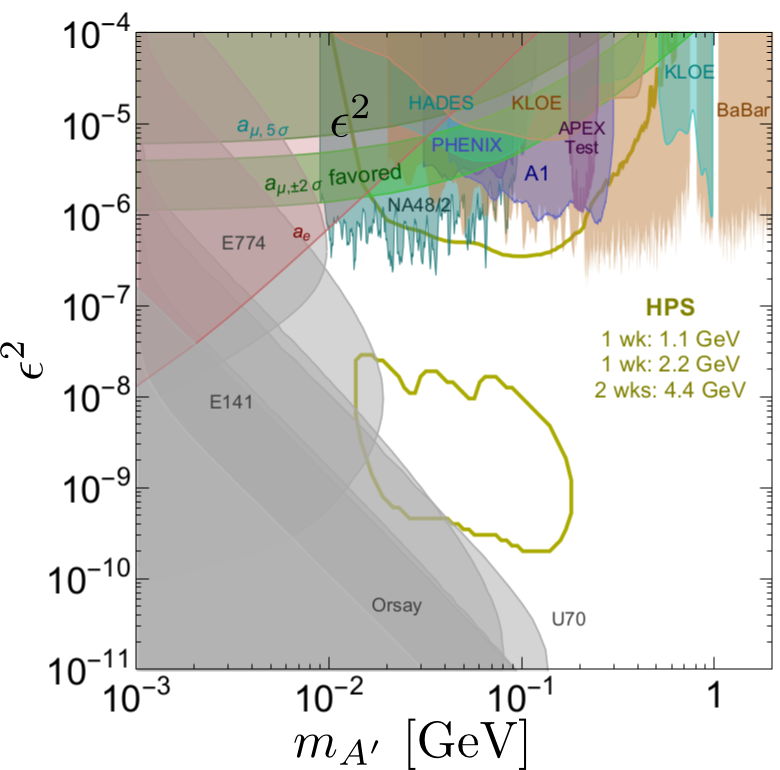
\includegraphics[width=0.9\textwidth]{images/ap_current_limits.png}
    \caption{Current limits on heavy photons.}
    \label{fig:svt_layout_render}
\end{figure}
